\documentclass[border=8pt,tikz]{standalone}
\usepackage{amsmath,amssymb}
\usepackage{tikz}
\usetikzlibrary{arrows.meta,calc,decorations.pathreplacing,patterns,shapes.geometric,positioning,shadings,plotmarks}

\begin{document}
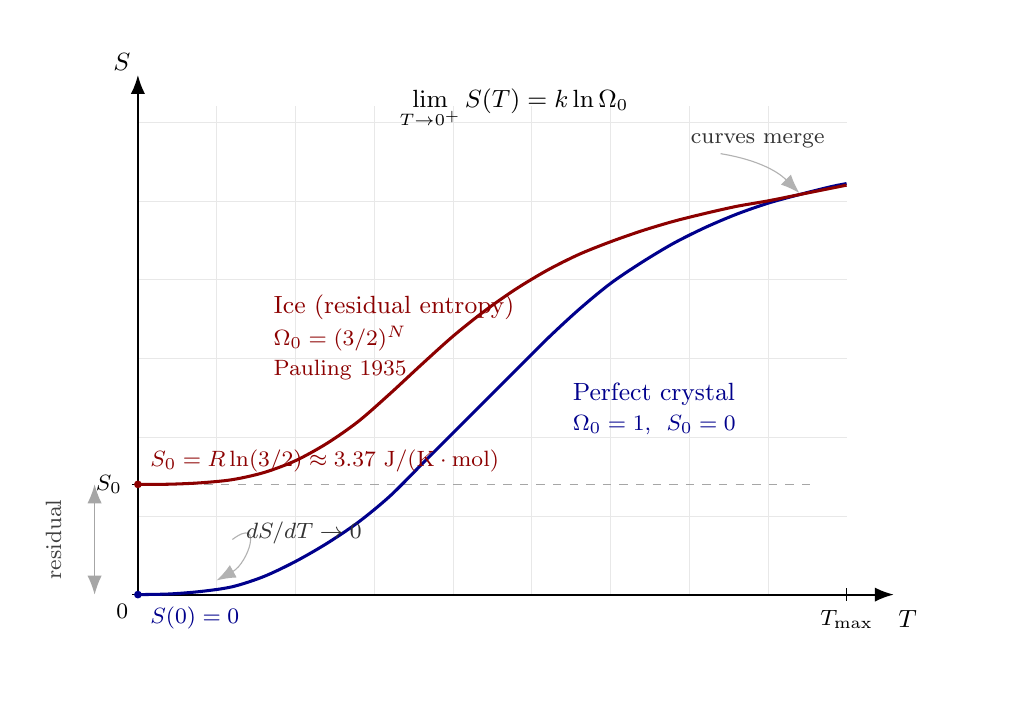
\begin{tikzpicture}[>={Latex[length=2.4mm]},x=1cm,y=1cm]

% --- Frame parameters ---
% Horizontal axis: T from 0 to 9 (cm), representing 0..T_max
% Vertical axis: S from 0 to 6 (cm)
% Residual entropy S_0 (ice) at y = 1.4 cm
% Both curves merge near (T = 7..9, S = 5.0..5.4)

% --- Background ---
\fill[white] (-1.4,-1.2) rectangle (10.8,7.2);

% --- Light grid ---
\foreach \x in {1,2,3,4,5,6,7,8}{%
  \draw[gray!18,very thin] (\x,0) -- (\x,6.2);
}
\foreach \y in {1,2,3,4,5,6}{%
  \draw[gray!18,very thin] (0,\y) -- (9,\y);
}

% --- Axes ---
\draw[->,line width=0.7pt,black] (0,0) -- (9.6,0) node[below right=2pt and -2pt,font=\small] {$T$};
\draw[->,line width=0.7pt,black] (0,0) -- (0,6.6) node[above left=-2pt and -1pt,font=\small] {$S$};

% Origin label
\node[below left,font=\footnotesize] at (0,0) {$0$};

% T-axis tick at T_max
\draw (9,0.08) -- (9,-0.08) node[below,font=\footnotesize] {$T_{\max}$};

% S-axis: residual entropy S_0
\draw[dashed,gray!70] (0,1.4) -- (8.6,1.4);
\draw (0.08,1.4) -- (-0.08,1.4) node[left,font=\footnotesize] {$S_0$};
\draw (0.08,0) -- (-0.08,0);

% --- Perfect crystal curve: deep blue ---
% S(T) starts at 0, rises with T^3 curvature at low T,
% then merges with ice curve near high T.
% Sample points (T, S):
%   (0,0), (0.6,0.02), (1.2,0.10), (1.8,0.30), (2.4,0.65),
%   (3.0,1.10), (3.6,1.65), (4.2,2.25), (5.0,3.10), (6.0,3.95),
%   (7.0,4.60), (8.0,5.05), (9.0,5.30)
\draw[line width=1.1pt,blue!55!black,smooth]
  plot coordinates {
    (0,0) (0.4,0.008) (0.8,0.04) (1.2,0.10) (1.6,0.23)
    (2.0,0.42) (2.4,0.65) (2.8,0.92) (3.2,1.25) (3.6,1.65)
    (4.0,2.05) (4.4,2.45) (4.8,2.85) (5.2,3.25) (5.6,3.62)
    (6.0,3.95) (6.4,4.22) (6.8,4.46) (7.2,4.66) (7.6,4.83)
    (8.0,4.97) (8.4,5.08) (8.8,5.18) (9.0,5.22)
  };

% --- Ice curve: ochre/brown red ---
% Starts at S_0 = 1.4, then rises and merges with crystal curve.
% Sample points (T, S):
%   (0,1.4) flat for very small T (dS/dT -> 0),
%   then climbs to merge.
\draw[line width=1.1pt,red!55!black,smooth]
  plot coordinates {
    (0,1.40) (0.4,1.402) (0.8,1.42) (1.2,1.46) (1.6,1.55)
    (2.0,1.70) (2.4,1.92) (2.8,2.20) (3.2,2.55) (3.6,2.92)
    (4.0,3.28) (4.4,3.60) (4.8,3.88) (5.2,4.12) (5.6,4.32)
    (6.0,4.48) (6.4,4.62) (6.8,4.74) (7.2,4.84) (7.6,4.93)
    (8.0,5.00) (8.4,5.08) (8.8,5.16) (9.0,5.20)
  };

% --- Endpoint markers ---
% Perfect crystal endpoint at origin
\fill[blue!55!black] (0,0) circle (1.4pt);
\node[below right=1pt and 1pt,font=\footnotesize,blue!55!black] at (0,0) {$S(0)=0$};

% Ice endpoint at S_0
\fill[red!55!black] (0,1.4) circle (1.4pt);
\node[above right=1pt and 1pt,font=\footnotesize,red!55!black] at (0,1.4)
  {$S_0=R\ln(3/2)\approx 3.37\ \mathrm{J/(K\cdot mol)}$};

% --- Curve labels ---
\node[blue!55!black,font=\small,anchor=west] at (5.4,2.55)
  {Perfect crystal};
\node[blue!55!black,font=\footnotesize,anchor=west] at (5.4,2.15)
  {$\Omega_0 = 1$,\ \ $S_0 = 0$};

\node[red!55!black,font=\small,anchor=west] at (1.6,3.65)
  {Ice (residual entropy)};
\node[red!55!black,font=\footnotesize,anchor=west] at (1.6,3.25)
  {$\Omega_0 = (3/2)^N$};
\node[red!55!black,font=\footnotesize,anchor=west] at (1.6,2.85)
  {Pauling 1935};

% --- Master third-law statement ---
\node[font=\small,anchor=north west] at (3.2,6.55)
  {$\displaystyle \lim_{T\to 0^+} S(T) = k\ln \Omega_0$};

% --- Highlight the gap at T=0 ---
\draw[<->,gray!70,thin] (-0.55,0) -- (-0.55,1.4);
\node[gray!50!black,font=\footnotesize,rotate=90,anchor=south] at (-0.85,0.7)
  {residual};

% --- Annotation: low-T behavior ---
\draw[->,gray!60,thin] (1.2,0.7) .. controls (1.6,1.0) and (1.4,0.4) .. (1.0,0.18);
\node[gray!40!black,font=\footnotesize,anchor=west] at (1.25,0.78)
  {$dS/dT \to 0$};

% --- Annotation: merging at high T ---
\draw[->,gray!60,thin] (7.4,5.6) .. controls (8.0,5.5) and (8.2,5.3) .. (8.4,5.10);
\node[gray!40!black,font=\footnotesize,anchor=south west] at (6.9,5.55)
  {curves merge};

\end{tikzpicture}
\end{document}
